\chapter{Desenvolvimento}

Este capítulo discute o funcionamento dos algoritmos desenvolvidos para a coordenação da \rssf em conjunto com 
\vants. As próximas seções descrevem o problema tratado e apresentam soluções para a resolução destes problemas.


\section{Descrição do Problema}

Este trabalho preocupa-se em pesquisar e desenvolver estratégias para a
coordenação de uma rede de sensores heterogênea. A rede em questão deve ser
utilizada para prover tarefas de monitoramento e vigilância de um ambiente de
interesse. Como ferramentas para se realizar estas tarefas de monitoramento são
utilizados nós sensores terrestres equipados com diversas interfaces de
sensoriamento e \vants também equipados com interfaces de sensoriamento e
enlaces de comunicação sem fio.

A justificativa e motivação para a utilização destes diferentes tipos de nós
sensores encontra-se no fato de que um nó sensor terrestre usual apresenta
capacidade computacional reduzida. Portanto, estes tipos de nós são incapazes de
cumprir todas as tarefas da rede individualmente. Em contrapartida, estes nós
sensores convencionais geralmente possuem custos reduzidos, o que propicia o uso
de vários sensores para a realização de missões. 

\uavs podem variar em tamanhos, formas, configurações e propósitos, adequando-se
a diversos cenários de aplicação. Neste trabalho, justifica-se o uso de
\emph{Mini-UAVs} (UAVs Multi-Missão), que são aeronaves de custo não tão elevado
quando comparados aos custos de aeronaves de grande porte. Portanto, uma
alternativa interessante é a utilização de \emph{Mini-UAVs} carregando uma
variedade de sensores específicos (sensores como câmeras de alta resolução,
infra-vermelho, GPS, etc) e que possuam poder computacional superior aos nós
sensores terrestres, permitindo assim que os \vants possam realizar missões e
medidas mais sensíveis e específicas.

Esta relação entre sensores terrestres simples e de baixo custo e \vants
relativamente mais caros justifica o uso de vários sensores simples espalhados
pela área de interesse em conjunto com alguns poucos, ou apenas um, \vant para
realizar as tarefas mais específicas. 

Por fim, o problema tratado é o desenvolvimento de estratégias eficientes para detecção de um evento através dos
nós sensores mais simples e garantir que as mensagens sejam entregues aos \vants
mais hábeis a tratar o evento de forma específica.

Dentre uma infinidade de exemplos de monitoramento de áreas de interesse,
podem ser citados:

\begin{description}
 \item [Áreas Militares de Acesso Restrito:] Locais de acesso proibido, onde se deseja detectar a presença de intrusos.
 \item [Detecção de Fenômenos Físicos:] São áreas onde se pretende detecctar a ocorrência de fenômenos como alteração de
temperatura, umidade, sons, etc.
 \item [Observação de Animais:] Aplicações em que o objetivo seja o monitoramento de espécies de animais, como, por exemplo,
a presença de uma espécie incomum em uma determinada área.
\end{description}

% A figura \ref{fig:app} demonstra um exemplo do funcionamento básico do sistema de monitoramento.
% 
% \begin{figure}[h!]
% \centering
% 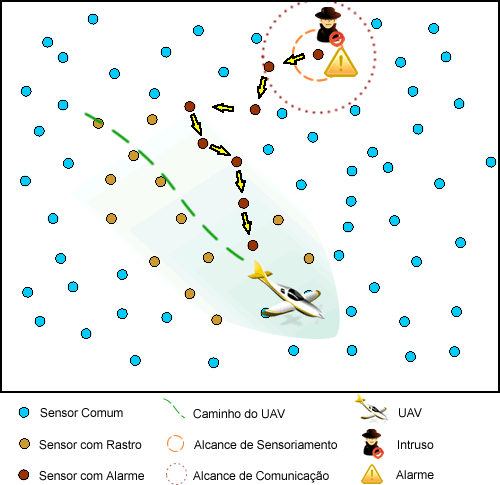
\includegraphics[width=12cm]{pictures/application.png}
% \caption{Funcionamento Básico da Aplicação}
%  \label{fig:app}
% \end{figure}


Observados os problemas e exemplos expostos anteriormente, este trabalho apresenta algumas soluções para se aprimorar
a utilização de veículos aéreos não tripulados em conjunto com redes de sensores sem fio.

Resumidamente, os algoritmos desenvolvidos são:

\begin{description}

	\item[ (a) Distribuição de Ferormônio: ] o \vant sobrevoa continuamente
a área de interesse da aplicação. Enquanto sobrevoa esta área, o \vant deve se
comunicar com os nós sensores que se encontram abaixo do mesmo, estes nós
armazenam um valor com a intensidade do sinal com que a mensagem foi recebida.
Neste momento é formado um gradiente que corresponde a um rastro artificial da aeronave.

	\item[ (b) Reforço dos Rastros de Ferormônio:] Em situações em que se utiliza mais de uma aeronave pode se 
tornar interessante desenvolver uma política de reforço dos rastros de ferormônio construídos em (a) por cada \vant.
Nesse caso, cada \vant pode reforçar o gradiente de todos os outros, desde que seus rastros se encontrem em algum ponto
da área de interesse.
	
	\item[ (c) Detecção e Propagação do Evento:] quando um evento é
detectado, os nós sensores terrestres devem realizar uma negociação a fim de
enviar uma mensagem de alarme para os \vants presentes na área. Esta mensagem
deve encontrar o rastro de ferormônio formado em (a) e (b) e prosseguir até o \vant
mais hábil para tratar o evento ocorrido.


%% Este aqui vai par os trabalhos futuros

% 	\item[ (c) \emph{Tracking} e Perseguição do Intruso: ] no momento em que
% os nós sensores detectam a presença de um dado evento, como exemplo o caso de um
% intruso, providências devem ser tomadas para que o mesmo alarme de evento não
% seja repetido. Por exemplo, o nó sensor X percebe a presença de um intruso na
% área, poucos segundos depois o nó Y também percebe o mesmo intruso, se ambos os
% nós enviarem um alarme aos \vants pode ocorrer carga excessiva na rede, bem como
% gerar confusão entre os \vants, pois os mesmos são interrompidos e reprogramados
% a cada alarme recebido. Portanto, na ocorrência de um evento, os nós da micro
% região onde onde houve a detecção devem alterar seu modo de trabalho, realizando
% assim uma perseguição e rastreamento, marcando uma trilha de mobilidade do
% evento, ao invés de soar os alarmes novamente.

\end{description}

As próximas seções discutem o problema apresentado em diferentes perspectivas, apresentando suas peculiaridades e possíveis
soluções.



